% =====================================================================
% CHEP 2026 poster: A Graph-Pipeline Framework for ALICE MC in Run 3
% A0 portrait, beamerposter + tcolorbox.
% Build: make   (or: pdflatex poster.tex, twice if refs change)
% =====================================================================
\documentclass[final,t]{beamer}
\usepackage[orientation=portrait,size=a0,scale=1.05]{beamerposter}

\usepackage[utf8]{inputenc}
\usepackage[T1]{fontenc}
\usepackage{amsmath}
\usepackage{amssymb}
\usepackage{lmodern}
\usepackage{helvet}
\renewcommand{\familydefault}{\sfdefault}

\usepackage{graphicx}
\usepackage{tcolorbox}
\tcbuselibrary{skins}
\usepackage{xcolor}
\usepackage{qrcode}
\usepackage{booktabs}
\usepackage{listings}
\usepackage{tikz}
\usetikzlibrary{tikzmark}
\usepackage{array}

\graphicspath{{Figs/}{Figs/CERNlogo/Outline/Formats PAO/}{../CHEP26Proceedings/Figs/}}

% ---------- Beamer plumbing ----------
\usetheme{default}
\setbeamertemplate{navigation symbols}{}
\setbeamertemplate{headline}{}
\setbeamertemplate{footline}{}
\setbeamercolor{background canvas}{bg=white}
\setbeamersize{text margin left=20mm,text margin right=20mm}

% ---------- Colour palette ----------
\definecolor{cernblue}{HTML}{0033A0}
\definecolor{cernbluedark}{HTML}{002677}
\definecolor{alicered}{HTML}{CC0033}
\definecolor{lightblue}{HTML}{EAF2FB}
\definecolor{lightred}{HTML}{FBEAEC}
\definecolor{rulegrey}{HTML}{B0B0B0}
\definecolor{textdark}{HTML}{1A1A1A}
\definecolor{jsongreen}{HTML}{1B5E20}

\setbeamercolor{normal text}{fg=textdark}
\setbeamercolor{itemize item}{fg=cernblue}
\setbeamercolor{itemize subitem}{fg=cernblue}
\setbeamercolor{enumerate item}{fg=cernblue}

% ---------- tcolorbox styles ----------
\tcbset{
  posterblock/.style={
    enhanced,
    arc=8mm, outer arc=8mm,
    boxrule=1.6pt,
    left=10mm, right=10mm, top=4mm, bottom=4mm,
    fonttitle=\bfseries\Large,
    coltitle=white,
    toptitle=4mm, bottomtitle=4mm, lefttitle=8mm,
    title style={opacity=1.0},
  }
}

\newtcolorbox{infoblock}[2][]{
  posterblock,
  colback=lightblue,
  colframe=cernblue,
  colbacktitle=cernblue,
  title=#2, #1,
}

\newtcolorbox{resultblock}[2][]{
  posterblock,
  colback=lightred,
  colframe=alicered,
  colbacktitle=alicered,
  title=#2, #1,
}

% ---------- Listings (JSON snippet) ----------
\lstdefinestyle{jsonstyle}{
  basicstyle=\ttfamily\small\color{textdark},
  showstringspaces=false,
  breaklines=true,
  columns=fullflexible,
  keepspaces=true,
  frame=none,
  aboveskip=2mm,
  belowskip=0mm,
  escapeinside={(*}{*)},
}

% ---------- Helpers ----------
% Render the logo if a file is present, otherwise a placeholder box.
\newcommand{\maybelogo}[3]{%
  \IfFileExists{#1}{\includegraphics[#2]{#1}}{%
    \setlength{\fboxrule}{1.5pt}\setlength{\fboxsep}{4mm}%
    \fcolorbox{rulegrey}{white}{\parbox[c][7cm][c]{\dimexpr\linewidth-15mm\relax}{\centering%
      \LARGE\color{rulegrey}\textsc{#3 logo}\\[2mm]%
      \small\color{rulegrey}(drop file here)}}%
  }%
}

\newcommand{\headlinerule}{\noindent\textcolor{cernblue}{\rule{\linewidth}{2.5pt}}}

% =====================================================================
\begin{document}
\begin{frame}[t,fragile]

\vspace*{2cm}

% ---------------- HEADER ----------------
\noindent\begin{minipage}[c]{0.15\linewidth}\centering
  
\includegraphics[height=9cm]{LogoOutline-Bleu.pdf}
\end{minipage}\hfill
\begin{minipage}[c]{0.68\linewidth}\centering
  {\color{cernblue}\bfseries\VeryHuge A Graph-Pipeline Framework for}\\[6mm]
  {\color{cernblue}\bfseries\VeryHuge ALICE Monte~Carlo in Run\,$\geq$\,3}\\[12mm]
  {\huge\bfseries Sandro Wenzel}\;{\Large\itshape for the ALICE Collaboration}\\[4mm]
  {\large CERN, Geneva, Switzerland \qquad\textbullet\qquad CHEP 2026}%
  \quad\smash{\raisebox{-0.35\height}{
\includegraphics[height=2.2cm]{CHEPBangkok_logo.jpeg}}}
\end{minipage}\hfill
\begin{minipage}[c]{0.15\linewidth}\centering
  
\includegraphics[height=9cm]{ALICE_logo.png}
\end{minipage}

\vspace{10mm}
\headlinerule
\vspace{12mm}

% ---------------- BODY: three columns ----------------
\begin{columns}[t,onlytextwidth]

% ============ COLUMN 1: Problem + Model ============
\begin{column}{0.318\textwidth}

\begin{infoblock}{1.~EPN\,$\leftrightarrow$\,Grid gap for MC}
Run~3 ships ALICE's novel \textbf{O\textsuperscript{2} Data
Processing Layer (DPL)}\,---\,an asynchronous, message-passing
framework running the \textbf{same reconstruction algorithms} online
(data taking) and offline.

\vspace{3mm}
\centering
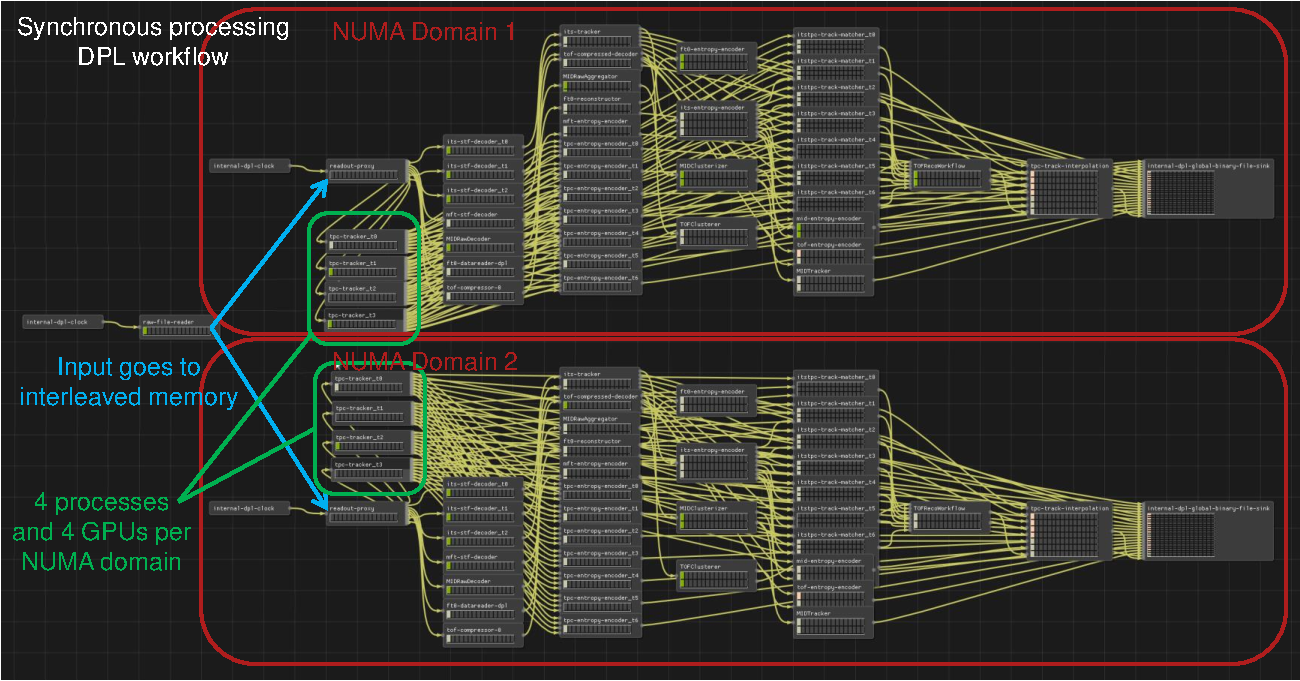
\includegraphics[width=\linewidth]{workflow-crop.pdf}\\[1mm]
{\small\itshape Excerpt of an actual DPL data-taking workflow on an EPN server.}\\[4mm]

\raggedright
\textbf{EPN servers:} $\geq 64$\,cores, hundreds of GB RAM, GPUs.\\[1mm]
\textbf{WLCG Grid slots:} \textbf{8\,cores / 16\,GB}.\\[2mm]
MC production layers simulation, digitisation and QC \emph{on top}\,---\,the monolithic
topology \textbf{does not fit}.

\vspace{5mm}
\noindent\colorbox{cernblue}{%
  \parbox{\dimexpr\linewidth-2\fboxsep\relax}{\centering
    \color{white}\large\bfseries
    How to run this on memory-constrained Grid sites\,---\,%
    \emph{optimally}\,?\strut
  }%
}
\end{infoblock}

\vspace{8mm}

\begin{infoblock}{2.~From DPL topology to a DAG}
\centering
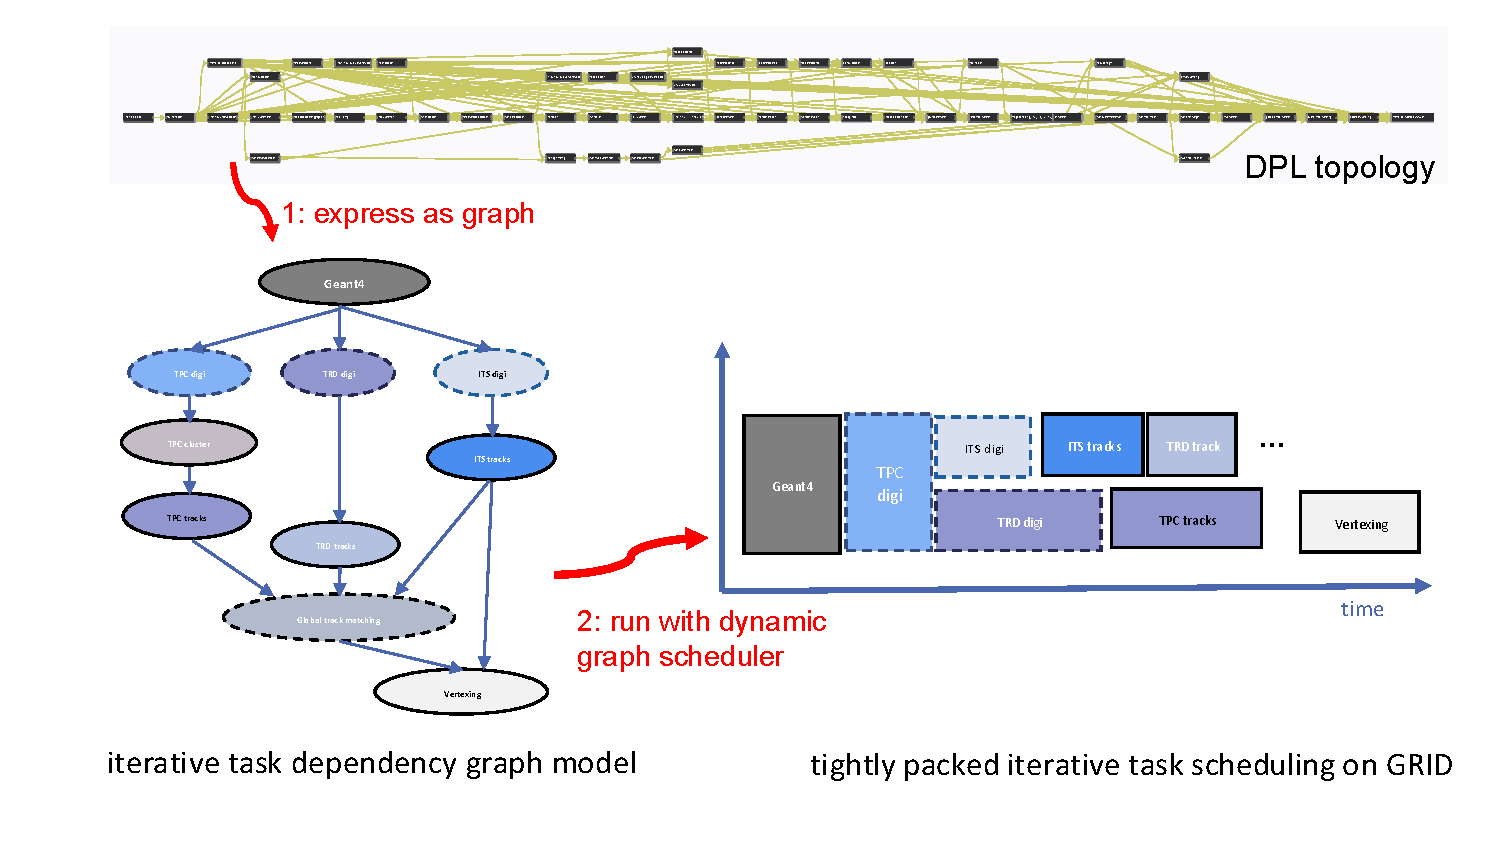
\includegraphics[width=\linewidth]{GraphApproachPoster.pdf}\\[3mm]
\raggedright
We express the simultaneous DPL topology as an \textbf{iterative DAG
of coarse-grained sub-tasks}, augmented with the extra MC stages
(event generation, transport, digitisation, $\dots$).

\vspace{3mm}
\textbf{Core idea:} execute the DAG along a topological order under
\textbf{explicit CPU and memory budgets}\,---\,only a small concurrent
subset of tasks is ever live, keeping the slot within limits.

\vspace{3mm}
\textbf{Additional benefits:}
\begin{itemize}\setlength\itemsep{1mm}
  \item nodes may be a DPL sub-topology, an O\textsuperscript{2}
        executable, or a script in any language;
  \item edges are data \texttt{needs}; files exchange via the local
        working directory\,---\,trivial restart and partial reruns.
\end{itemize}
\end{infoblock}

\vspace{8mm}

\begin{infoblock}{3.~Graph generation \& configuration}
A dedicated tool, \texttt{o2dpg\_sim\_workflow.py}, generates the
full Run\,3 MC workflow graph from physics-level inputs (collision
system, energy, generator, $N$ timeframes, $\dots$). The result is
serialised as JSON\,---\,one entry per task:

\vspace{3mm}
\noindent
\begin{minipage}{0.58\linewidth}
\begin{lstlisting}[style=jsonstyle]
{
 "name": "tpcdigi_tf1",(*\tikzmark{m-name}*)
 "cmd":  "o2-sim-digi...",
 "needs": ["sim_tf1","geo"],(*\tikzmark{m-needs}*)
 "resources":
   {"cpu":1,"mem":2000},(*\tikzmark{m-res}*)
 "software_package":
   "O2::v1.5.0",(*\tikzmark{m-sw}*)
 "timeframe": 1(*\tikzmark{m-tf}*)
}
\end{lstlisting}
\end{minipage}%
\begin{tikzpicture}[remember picture, overlay,
                    every node/.style={anchor=west,font=\small\bfseries}]
\node[text=cernblue] at ([xshift=5mm]pic cs:m-name)  {$\leftarrow$ task id};
\node[text=cernblue] at ([xshift=5mm]pic cs:m-needs) {$\leftarrow$ DAG edges};
\node[text=alicered] at ([xshift=5mm]pic cs:m-res)   {$\Leftarrow$ scheduling input};
\node[text=cernblue] at ([xshift=5mm]pic cs:m-sw)    {$\leftarrow$ per-task env};
\node[text=cernblue] at ([xshift=5mm]pic cs:m-tf)    {$\leftarrow$ timeframe id};
\end{tikzpicture}

\vspace{8mm}

\textbf{\texttt{resources} drives admission.}
Each task declares a peak-CPU (cores) and peak-memory (MB) estimate;
the scheduler runs only the subset that fits the slot budget.

\vspace{5mm}

\noindent\colorbox{cernblue}{%
  \parbox{\dimexpr\linewidth-2\fboxsep\relax}{\centering
    \color{white}\bfseries
    Defaults can be replaced by \emph{learned} values from a pilot run
    (\S7)\,---\,major makespan gains (\S8).\strut
  }%
}
\end{infoblock}

\vfill

% ---- footer block: QR, references, contact (anchored to column bottom) ----
\noindent\textcolor{cernblue}{\rule{\linewidth}{2pt}}\\[3mm]

\noindent
\begin{minipage}[c]{5.5cm}\centering
  \qrcode[height=5cm]{https://github.com/AliceO2Group/O2DPG}\\[1mm]
  {\scriptsize O2DPG on GitHub}
\end{minipage}\hfill
\begin{minipage}[c]{\dimexpr\linewidth-5.5cm-5mm\relax}\footnotesize
\textbf{References.}\,
[1]~ALICE Coll., \emph{O\textsuperscript{2} TDR}, CERN-LHCC-2015-006 (2015).\,
[2]~G.~Eulisse \emph{et al.}, ALICE DPL, CHEP 2018.\,
[3]~H.~Topcuoglu \emph{et al.}, IEEE TPDS \textbf{13}, 260 (2002) (HEFT).\,
[4]~F.~M\"older \emph{et al.}, F1000Research \textbf{10}, 33 (2021).\\[2mm]
\textbf{Contact:}\; sandro.wenzel@cern.ch\quad\textbullet\quad CERN, Geneva
\end{minipage}

\end{column}

% ============ COLUMN 2: The engine ============
\begin{column}{0.318\textwidth}

\begin{infoblock}{4.~Workflow runner}
A dedicated Python runner \textbf{executes the graph by
topological-order analysis}, in a steady-state loop:
\begin{enumerate}\setlength\itemsep{1mm}
  \item maintain the ready set (tasks whose \texttt{needs} are done),
  \item order candidates by the active scheduling policy,
  \item admit those that fit the CPU and memory budget,
  \item monitor execution; on completion mark done and continue.
\end{enumerate}
\vspace{2mm}
\textbf{Process isolation} per task $=$ fault containment $+$ language
$+$ software-tag mixing.\\[1mm]
\textbf{Start-stop-resume:} sentinel files for already-completed tasks
enable seamless restart after Grid preemption, targeted partial
re-runs, and incremental development.
\end{infoblock}

\vspace{8mm}

\begin{infoblock}{5.~Three scheduling policies}
The runner is configurable with different \textbf{task-ordering
strategies} for the ready set:
\begin{itemize}\setlength\itemsep{2mm}
  \item \textbf{Timeframe-first}\,---\,drain small-index timeframes
        first; within a timeframe, prefer the most-connected task.
  \item \textbf{Best-fit bin-packing}\,---\,maximise
        $f = \mathrm{cp}(t)\cdot\max(c/c_{\text{free}},\,m/m_{\text{free}})$.
  \item \textbf{Critical-path (HEFT-inspired)}\,---\,order by the
        remaining longest path to a leaf, weighted by learned walltime.
        \textbf{Empirically the best} once measurement informs the
        weights.
\end{itemize}
\end{infoblock}

\vspace{8mm}

\begin{infoblock}{6.~Backfilling: the wall-time lever}
\textbf{Two-lane admission}, shared by every policy:
\begin{itemize}\setlength\itemsep{1mm}
  \item \textbf{Default lane:} book CPU and memory within the hard
        slot budget.
  \item \textbf{Backfill lane:} admit additional low-priority (niced)
        tasks with a bounded over-commit on top of the default lane.
\end{itemize}
Linux's CFS automatically demotes the niced backfill tasks whenever
the default lane needs CPU\,---\,backfill silently \emph{fills the CPU
holes} between heavyweight stages.

\vspace{3mm}
\centering
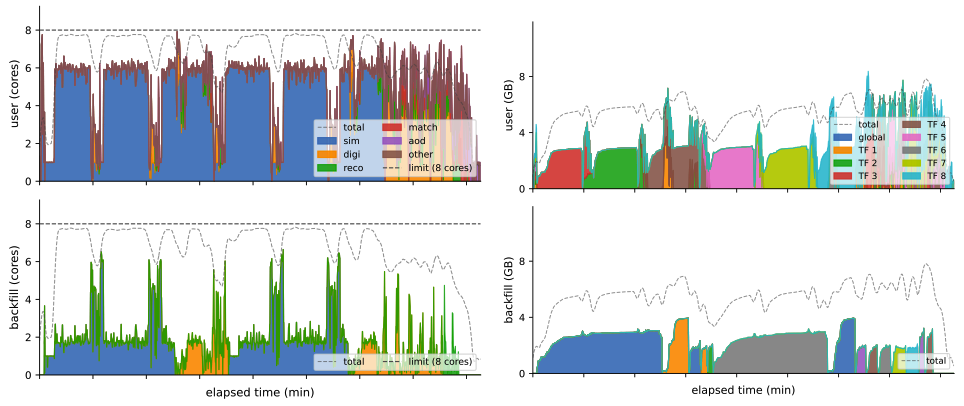
\includegraphics[width=\linewidth]{CPUandMemUserAndBackfill.png}\\[1mm]
{\small\itshape CPU utilisation and task allocation vs.\ time, split
into default lane (top) and backfill lane (bottom), for CPU (left) and
memory (right). Backfill fills the CPU holes; the 16\,GB memory
budget (dashed) is respected.}\\[3mm]

\colorbox{cernblue}{\color{white}\large\bfseries~~Removes
$\sim 20\%$ of makespan~~}
\end{infoblock}

\vspace{8mm}

\begin{infoblock}{7.~Pilot-guided MC campaigns}
For any large MC campaign we recommend an \emph{optional but
natural} preparation step: a short reference run on representative
input that primes the framework for high-CPU-efficiency
production.

\vspace{2mm}
The pilot delivers three reusable artefacts at once:
\begin{enumerate}\setlength\itemsep{1mm}
  \item \textbf{Correctness gate} for the full campaign,
  \item \textbf{Resource profile} (measured CPU\,\& memory per task)
        $\rightarrow$ overrides the defaults (\S3),
  \item \textbf{File-artefact dependency graph} via \texttt{fanotify}
        \,---\,learns which task produces and which tasks consume each
        intermediate file, enabling aggressive early cleanup (\S10).
\end{enumerate}

\vspace{3mm}
\centering
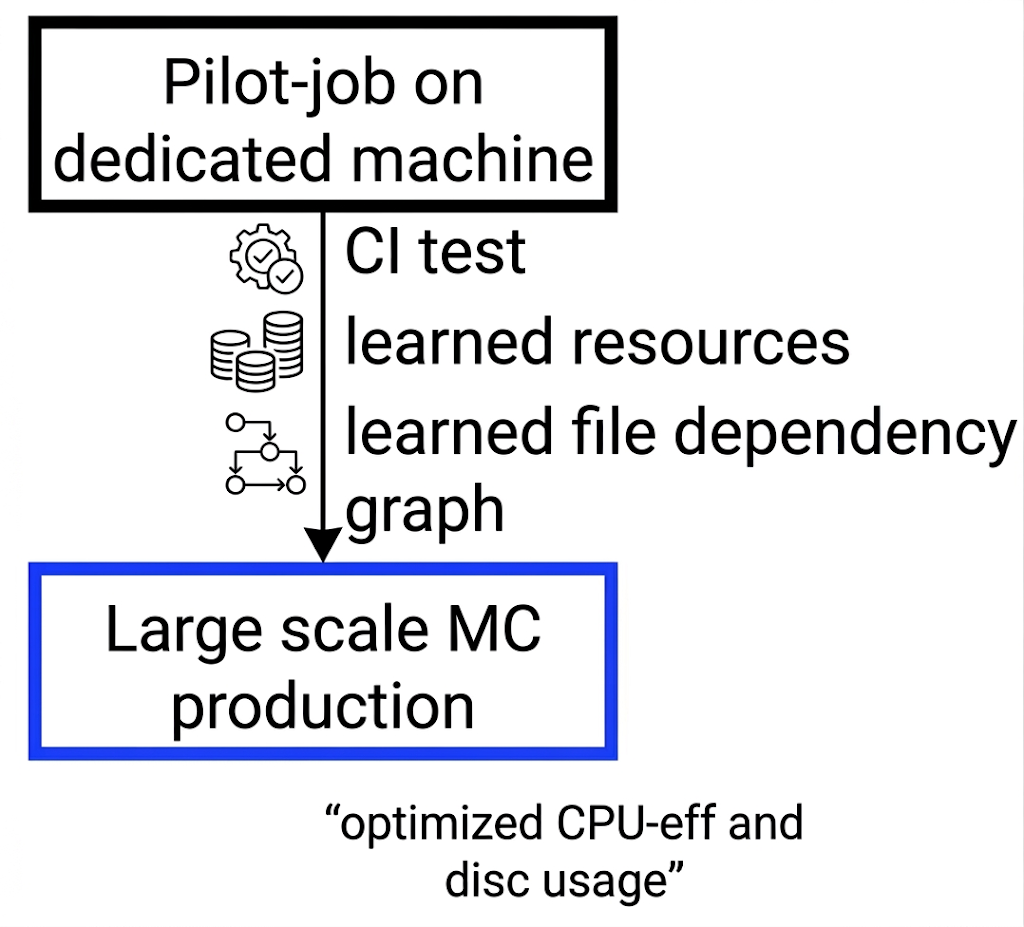
\includegraphics[width=0.75\linewidth]{pilot.png}
\end{infoblock}

\end{column}

% ============ COLUMN 3: Results + outlook ============
\begin{column}{0.318\textwidth}

\begin{resultblock}{8.~Quantitative results}
Benchmark: pp\,MC workflow, 8 timeframes ($\sim 200$ events each),
8-core / 16\,GB slot.\\[3mm]

\centering
\setlength{\tabcolsep}{8pt}
\renewcommand{\arraystretch}{1.2}
\begin{tabular}{lccc}
\toprule
                          & best-fit & timeframe & cp \\
\midrule
default, no backfill      & ---      & 3368      & ---  \\
default + backfill        & ---      & 2855      & ---  \\
\addlinespace
learned, no backfill      & 3157     & 3273      & 3118 \\
learned + backfill        & 2557     & 2598      &
                            {\bfseries\color{alicered}2482} \\
\bottomrule
\end{tabular}\\[3mm]

{\small Makespan in seconds; mean over multiple runs.}\\[6mm]

\begin{tikzpicture}[
  card/.style   ={fill=white, draw=alicered, line width=1.4pt,
                  rounded corners=3mm, inner sep=2.5mm,
                  minimum width=4.6cm, align=center,
                  font=\small\bfseries, text=alicered},
  banner/.style ={fill=alicered, text=white, rounded corners=5mm,
                  inner sep=4mm, font=\Large\bfseries,
                  minimum width=14cm, align=center},
  arr/.style    ={->, alicered, line width=1.6pt,
                  shorten >=1.5mm, shorten <=1.5mm}
]
  \node[card]   (c1) at (-7, 1.5) {Backfilling      \\[0.5mm] {\Large $\sim\!20\%$}};
  \node[card]   (c2) at ( 0, 1.5) {Resource learning\\[0.5mm] {\Large $\sim\!9\%$}};
  \node[card]   (c3) at ( 7, 1.5) {Critical-path    \\[0.5mm] {\Large $\sim\!5\%$}};
  \node[banner] (b)  at ( 0,-1.6) {26\,\% faster execution
                                   \\[0.5mm] {\normalsize 3368\,s $\rightarrow$ 2482\,s}};
  \draw[arr] (c1.south) to[out=-90,in=170] (b.west);
  \draw[arr] (c2.south) -- (b.north);
  \draw[arr] (c3.south) to[out=-90,in=10]  (b.east);
\end{tikzpicture}
\end{resultblock}

\vspace{8mm}

\begin{infoblock}{9.~Discrete-event schedule simulator}
A standalone tool simulates full workflow execution from the same
admission rules used at runtime, based on idealistic \emph{mean}
models of per-task CPU occupancy and backfill hole-filling. It
predicts \textbf{makespan} and \textbf{CPU efficiency} in
milliseconds.

\vspace{3mm}
\centering
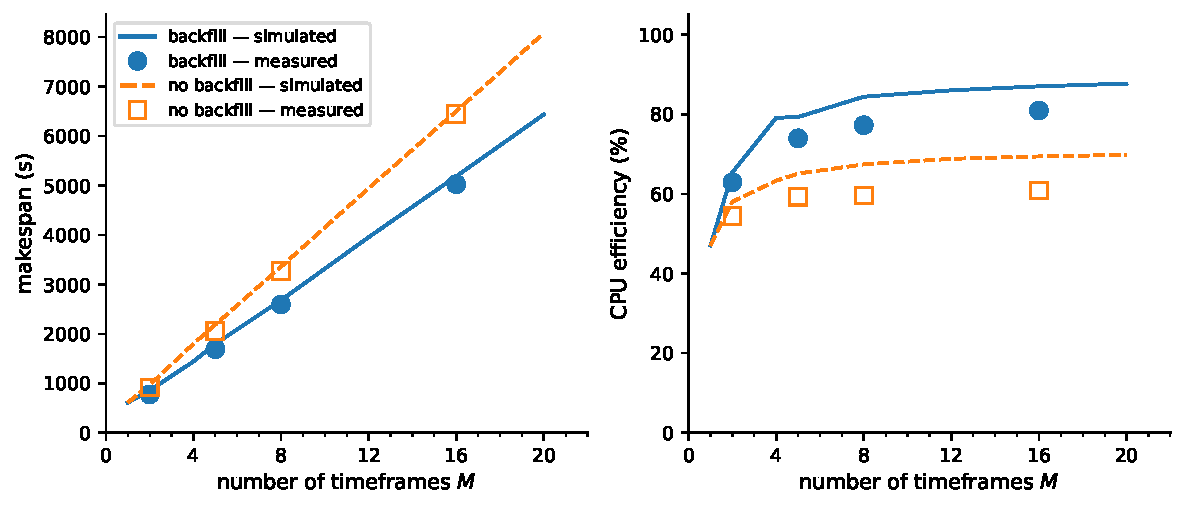
\includegraphics[width=\linewidth]{sim_vs_measured.pdf}\\[1mm]
\raggedright\small
No contention modelled\,---\,prediction is an upper bound\,---\,yet
measurement tracks within \textbf{5--10\,\%}.

\vspace{5mm}

\noindent\colorbox{cernblue}{%
  \parbox{\dimexpr\linewidth-2\fboxsep\relax}{\centering
    \color{white}\bfseries\large
    Ultra-fast lever for job dimensioning
    \,\textbullet\,\ CPU-efficiency prediction\strut
  }%
}
\end{infoblock}

\vspace{8mm}

\begin{infoblock}{10.~Active disc-space management}
The runner \textbf{deduces file-level relationships not expressed in
the original workflow graph}: a \texttt{fanotify} sidecar traces every
file read/write during the pilot, building a producer/consumer map of
all intermediate artefacts.

\vspace{2mm}
Production runs use this map to \textbf{actively reclaim scratch
space} as the workflow progresses\,---\,an intermediate file is
deleted the moment its last consumer has finished.

\vspace{3mm}
\centering
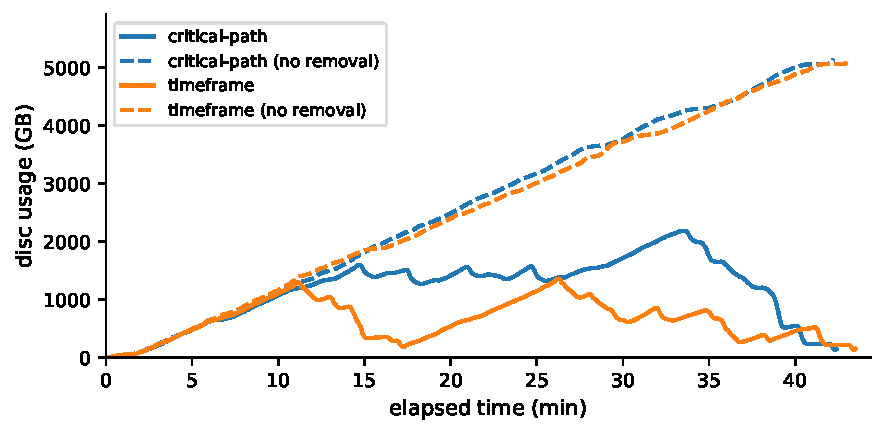
\includegraphics[width=0.8\linewidth]{disc_compare.pdf}\\[1mm]
\raggedright\small
On-disc footprint stays at the working-set size, not the cumulative
production size.

\vspace{4mm}

\noindent\colorbox{cernblue}{%
  \parbox{\dimexpr\linewidth-2\fboxsep\relax}{\centering
    \color{white}\bfseries
    Overcomes the few-tens-of-GB scratch limit of Grid slots.\strut
  }%
}
\end{infoblock}

\vspace{8mm}

\begin{resultblock}{11.~Conclusion}
A production-ready framework for ALICE Run\,3 MC. Headline benefits
on the same Grid slot:
\begin{itemize}\setlength\itemsep{1mm}
  \item \textbf{high CPU efficiency at low memory footprint}
        (vs.\ a monolithic DPL deployment) via dense scheduling
        and backfilling,
  \item per-task software environments\,---\,reconstruction and
        simulation can run on different release tags side by side,
  \item language-agnostic tasks (DPL, executables, scripts),
  \item active scratch-disc management,
  \item DAG-based execution: start-stop-go, fault-tolerant restart,
        easy partial reruns.
\end{itemize}

\vspace{4mm}
\noindent\colorbox{alicered}{%
  \parbox{\dimexpr\linewidth-2\fboxsep\relax}{\centering
    \color{white}\bfseries\Large
    Ability to execute MC workflows efficiently on the WLCG
    Grid.\strut
  }%
}
\end{resultblock}

\end{column}
\end{columns}

\end{frame}
\end{document}
